\documentclass[6pt,landscape]{article}
\usepackage{multicol}
\usepackage{calc}
\usepackage{ifthen}
\usepackage[landscape]{geometry}
\usepackage{amsmath,amsthm,amsfonts,amssymb}
\usepackage{color,graphicx,overpic}
\usepackage{hyperref}
\usepackage{gensymb}

\pdfinfo{
  /Title (example.pdf)
  /Creator (TeX)
  /Producer (pdfTeX 1.40.0)
  /Author (Seamus)
  /Subject (Example)
  /Keywords (pdflatex, latex,pdftex,tex)}

% This sets page margins to .5 inch if using letter paper, and to 1cm
% if using A4 paper. (This probably isn't strictly necessary.)
% If using another size paper, use default 1cm margins.
\ifthenelse{\lengthtest { \paperwidth = 11in}}
    { \geometry{top=.5in,left=.5in,right=.5in,bottom=.5in} }
    {\ifthenelse{ \lengthtest{ \paperwidth = 297mm}}
        {\geometry{top=1cm,left=1cm,right=1cm,bottom=1cm} }
        {\geometry{top=1cm,left=1cm,right=1cm,bottom=1cm} }
    }

% Turn off header and footer
\pagestyle{empty}

% Redefine section commands to use less space
\makeatletter
\renewcommand{\section}{\@startsection{section}{1}{0mm}%
                                {-1ex plus -.5ex minus -.2ex}%
                                {0.5ex plus .2ex}%x
                                {\normalfont\large\bfseries}}
\renewcommand{\subsection}{\@startsection{subsection}{2}{0mm}%
                                {-1explus -.5ex minus -.2ex}%
                                {0.5ex plus .2ex}%
                                {\normalfont\normalsize\bfseries}}
\renewcommand{\subsubsection}{\@startsection{subsubsection}{3}{0mm}%
                                {-1ex plus -.5ex minus -.2ex}%
                                {1ex plus .2ex}%
                                {\normalfont\small\bfseries}}
\makeatother

% Define BibTeX command
\def\BibTeX{{\rm B\kern-.05em{\sc i\kern-.025em b}\kern-.08em
    T\kern-.1667em\lower.7ex\hbox{E}\kern-.125emX}}

% Don't print section numbers
\setcounter{secnumdepth}{0}


\setlength{\parindent}{0pt}
\setlength{\parskip}{0pt plus 0.5ex}

%My Environments
\newtheorem{example}[section]{Example}
% -----------------------------------------------------------------------

\begin{document}
\raggedright
\footnotesize
\begin{multicols*}{5}


% multicol parameters
% These lengths are set only within the two main columns
%\setlength{\columnseprule}{0.25pt}
\setlength{\premulticols}{1pt}
\setlength{\postmulticols}{1pt}
\setlength{\multicolsep}{1pt}
\setlength{\columnsep}{2pt}

\begin{center}
     \Large{\underline{Sensor Principles}} \\
 
\end{center}


% Summary starts here
% --------------------------------------------------------------------------------------
\subsection{A generic sensor interface}
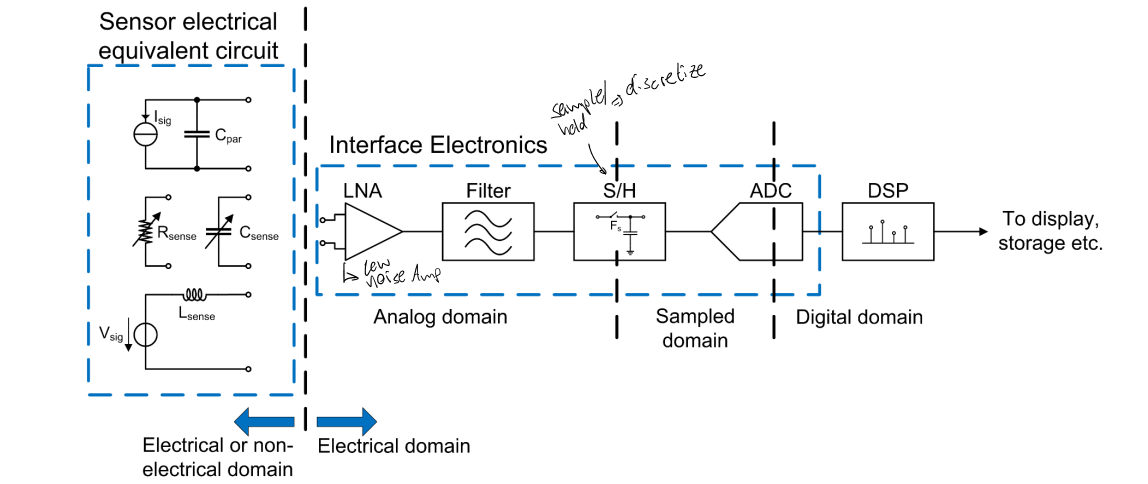
\includegraphics[width = \columnwidth]{images/generic_sensor_interface.png}
\subsection{OPAMP Basics}
\subsection{Opamps in feedback}
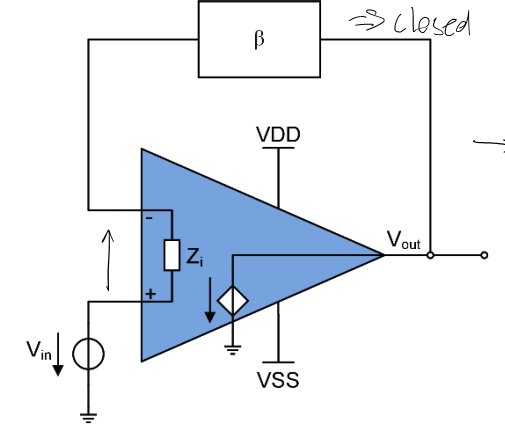
\includegraphics[width = \columnwidth]{images/opampfeedbacl.png}
Gain : $ T(\omega) =\beta \cdot A_0 (\omega $) \\
Phase Margin: $PM =180 \degree + \angle (T(\omega_1)|_{  |T(\omega_1)| = 1 } $
Gain margin:$ GM = 20 \cdot log_{10} (\frac{1}{T(\omega_2)})|_{\angle (T(\omega_2) = - 180 \degree  }$
\textbf{Generic Transfer function}\\
%$ Z_i \rightarrow \infty \Rightarrow V_X = \beta \cdot V_{out} = \beta  $
$  V_{x}=\beta \cdot V_{\text {out }}=\beta \cdot A(\omega) \cdot\left(V_{\text {in }}-V_{x}\right)=\beta \cdot A(\omega) \cdot\left(V_{\text {in }}-\beta \cdot V_{\text {out }}\right)$\\
$ \frac{V_{\text {out }}}{V_{\text {in }}}=\frac{A(\omega)}{1+\beta \cdot A(\omega)} \stackrel{A(\omega)] \gg 1}{\approx} \frac{1}{\beta} $
\textbf{Negative Feedback and linear operation}\\
$ A(\omega) \gg 1 \Rightarrow $ virtual short at the input $ \Delta V \approx 0  $ \\
$ Z_i \rightarrow \infty \Rightarrow i_{oa} \approx 0 $ \\
 Voltage Drive $ \rightarrow $ negative feedback\\
 Current drive $ \rightarrow $ positive feedback 
 \subsection{Errors and Noise}
 \textbf{Limit of detection(LOD):} minimum measurable input amplitude ($ SNR \approx 0 $)  \\
 \textbf{Dynamic range()DR:} ratio of max and min amplitude within inaccuracy levels.\\
 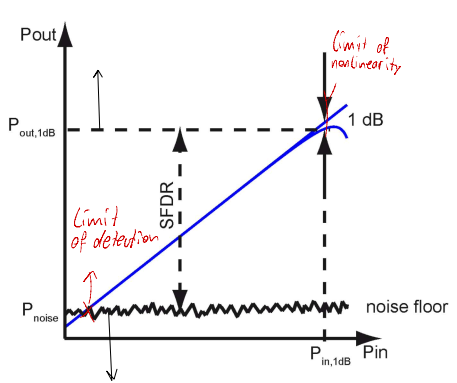
\includegraphics[width = \columnwidth]{images/lod_dr.png}\\
 \textbf{Errortypes}:\\
 Deterministic: source loading, offset, gain error \\
 Random: thermal noise, 1/f noise\\
 \textbf{Quantification}:\\
 Absolute : $ \Delta x=\left|\hat{x}-x_{0}\right| $\\
Relative: $\left|\frac{\Delta x}{x_{0}}\right|=\left|\frac{\hat{x}-x_{0}}{\hat{x}}\right|  $\\
Max inaccuracy: $ \Delta x_{max}| x \in \left[\hat{x}-\Delta x_{\max }, \hat{x}+\Delta x_{\max }\right] $
\textbf{Error Propagation}\\
$ y=f\left(x_{1}, x_{2}, \ldots, x_{N}\right) $\\
Deterministic fluctuations of $ x_i $ $ \rightarrow $ total error:\\
$\Delta y \approx \sum_{i=1}^{N} \frac{\partial f}{\partial x_{i}} \cdot \Delta x_{i}  $\\
Partial derivative $ \frac{\delta f}{\delta x_i} $ is called \textbf{sensitivity}\\
Additive errors are best specified absolute and multiplicative errors are best specified relative \\
\textbf{Interference:}\\
Unwanted coupling of external signal\\
Noise: random fluctuations from setup $ \rightarrow $ can be modeled as error sources
\subsection{Combining Error sources}
\textbf{Output referred noise}\\
Effect of an error-source on the output\\
\textbf{Input referred noise}
Equivalent effect of the error-source on the input\\
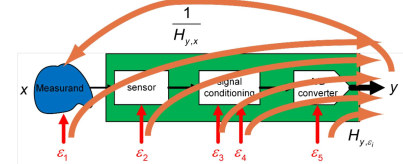
\includegraphics[width = \columnwidth]{images/error_referral.png}\\
Find TF from ES to output $ y:H_{y,ES} \Rightarrow y_{\text {out }, \epsilon_{2}}=H_{y, \epsilon_{2}} \cdot \epsilon_{2}$\\
Refer result back to input wit $ H_{y,x}: x_{\epsilon_{2}}=\frac{y_{\text {out }, \epsilon_{2}}}{H_{y, x}}=H_{y, \epsilon_{2}} \cdot \frac{\epsilon_{2}}{H_{y, x}} $\\
\textbf{Lin. System noise:}\\
$ PSD =  S_{y}(f)=|H(f)|^{2} \cdot S_{x}(f)$
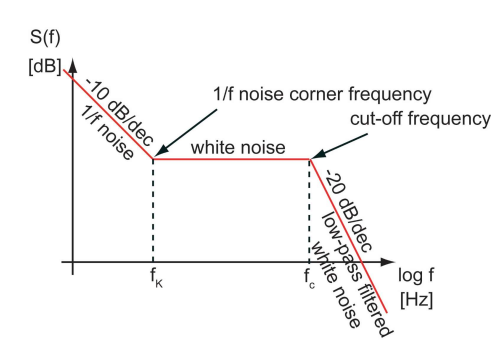
\includegraphics[width = \columnwidth]{images/noise_bode.png}
\subsection{Noise Types}
\textbf{Thermal noise:} excitation of charge carriers(white)\\
\textbf{Shot noise: }carriers randomly crossing the barrier, dependent on DC bias and white \\
\textbf{Flicker Noise:}, due to traps in semiconduct. 1/f spectral density. MOS trans at low freq.\\
\textbf{Thermalnoise Theorem:} Every closed system at temp. T has average. Energy of $ kT/2 $
$ \rightarrow $ $S_{u}(f)=2 k T R($ double-sided $)$ math
$S_{u}(f)=4 k T R($ single-sided $)$ physics
\subsection{Langevin Approach kt/C noise}
PSD noise voltage of $ V_n $ $ = S_{v_{n}}(f)=4 k T \cdot \Re\{Z(j 2 \pi f) $\\
$ \rightarrow $ $ \overline{V_{n}^{2}}=k T\left[\frac{1}{C_{\infty}}-\frac{1}{C_{0}}\right]=\frac{k T}{C} $\\
\textbf{MOS IRN}\\
$ S_{\Delta V_{\text {nG-tot }}^{2}}=4 k T \cdot R_{\text {nG-tot }}, \quad R_{\text {nG-tot }}=\frac{\rho}{W \cdot L \cdot f}+\frac{\gamma_{n D}}{G_{m}} $ with GateExcess Noise factor :$ \gamma_{n D} = (n=1.3) \cdot [0.5 WI; 2/3 SI] $ \\
\textbf{Bipolar Trans IRN:}\\
$ S_{\Delta V_{n R}^{2}}=4 k T \cdot R_{B} $
\subsection{Noise Aanalysis}
small-signal-equivalent is valid.\\
Total ORN: $ S_{n, \text { out }}(f)=\sum_{k=1}^{N}\left|H_{k}(f)\right|^{2} \cdot S_{n k}(f) $\\
N uncorrelated NS.\\
$ H_k(f) $ TF from NS ton output.
IRN: $ S_{V_{\text {neq,IRN }}}(f)=\frac{S_{V_{\text {nout }}}(f)}{|A(f)|^{2}} $ with $ A(f) $ is TF\\
\section{Sensor types}
Information domain $ \rightarrow $ Electrical domain\\
Transduction: Converting a signal from the energy domain into another.\\
Sensors and actuators are transducers\\
\subsection{Sources of eerror}
Noise, sensitivity to unintended quantities, Noise, EMI\\
%\texttt{$ \left(\begin{array}{c}
%E_{\operatorname{mag}} \\
%E_{\text {mech }} \\
%E_{\text {therm }} \\
%E_{\text {opt }} \\
%E_{\text {chem }} \\
%E_{\text {elec }}
%\end{array}\right)= \left(\begin{array}{cccccc}
%\alpha_{\text {mag,mag }} & \alpha_{\text {mag,mech }} & \alpha_{\text {mag,therm }} & \alpha_{\text {mag,opt }} & \alpha_{\text {mag,chem }} & \alpha_{\text {mag,elec }} \\
%\alpha_{\text {mech,mag }} & \alpha_{\text {mech,mech }} & \alpha_{\text {mech,therm }} & \alpha_{\text {mech,opt }} & \alpha_{\text {mech,chem }} & \alpha_{\text {mech,elec }} \\
%\alpha_{\text {therm,mag }} & \alpha_{\text {therm,mech }} & \alpha_{\text {therm,therm }} & \alpha_{\text {therm,opt }} & \alpha_{\text {therm,chem }} & \alpha_{\text {therm,elec }} \\
%\alpha_{\text {opt,mag }} & \alpha_{\text {opt,mech }} & \alpha_{\text {opt,therm }} & \alpha_{\text {opt,opt }} & \alpha_{\text {opt,chem }} & \alpha_{\text {opt,elec }} \\
%\alpha_{\text {chem,mag }} & \alpha_{\text {chem,mech }} & \alpha_{\text {chem,therm }} & \alpha_{\text {chem,opt }} & \alpha_{\text {chem,chem }} & \alpha_{\text {chem,elec }} \\
%\alpha_{\text {elec,mag }} & \alpha_{\text {elec,mech }} & \alpha_{\text {elec,therm }} & \alpha_{\text {elec,opt }} & \alpha_{\text {elec,chem }} & \alpha_{\text {elec,elec }}
%\end{array}\right) \cdot \left(\begin{array}{c}
%E_{\operatorname{mag}} \\
%E_{\text {mech }} \\
%E_{\text {therm }} \\
%E_{\text {opt }} \\
%E_{\text {chem }} \\
%E_{\text {elec }}
%\end{array}\right)+\left(\begin{array}{c}
%E_{\text {mag,os }} \\
%E_{\text {mech,os }} \\
%E_{\text {therm,os }} \\
%E_{\text {opt }, \mathrm{os}} \\
%E_{\text {chem }, \mathrm{os}} \\
%E_{\text {elec }, \mathrm{os}}
%\end{array}\right) $}
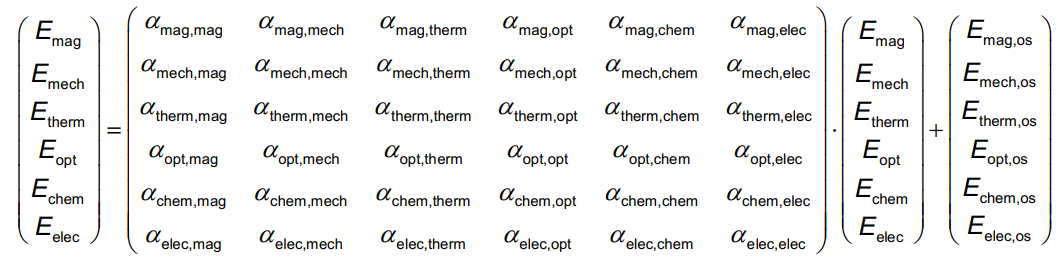
\includegraphics[width = \columnwidth]{images/transconduction_matrix.png}\\
Tandem transducers: Multiple steps to target domain.\\
cross-sensitivity, sensitivity to undesired quantity
\subsection{Sensor classification:}
\textbf{Active Sensors:}\\
Require external source of excitation\\
\textbf{Passive / self-generating sensors:}\\
Generate their own electrical output signal\\
Draws all required energy from the measurand(source loading)
E: Potentiometer for angle measurements.
\textbf{Modulating sensors:}\\
Measure desired quantity by modulating\\
Additional source with modulated energy. Also adds error.
E: Non0contact displacement measrement (rotating disk)
\textbf{Analog vs. Digital:}\\
Analog: time and value continuous\\
Digital: Discrete outputs\\
\textbf{Deflection mode sensors:}\\
Response to an output is a deviation from the equilibrium position\\
\textbf{Null mode sensors:}\\
Sensor or instruments exert an influence the measured system opposing the effect of the measurand. Ideally the result is a 0 measurement, typically achieved by feedback. The opposing influence is then the sensor output.
Slower than deflection, but more accurate.\\
\textbf{Resistive sensors - strain gauges}\\
Change in geometry under mechanical stress produces associated resistance change\\
Volum. == const. $ \rightarrow $ $ \frac{\partial V}{V_{0}}=\frac{L_{0}}{V_{0}} \cdot \partial A+\frac{A_{0}}{V_{0}} \cdot \partial L \wedge \frac{\partial V}{V_{0}}=0 \Rightarrow \frac{\partial A}{A_{0}}=-\frac{\partial L}{L_{0}}  $ $ \rightarrow $ $ \frac{\partial R}{R_{0}}=\frac{\partial \rho}{\rho_{0}}+2 \frac{\partial L}{L_{0}} $ $ \rightarrow $$ \frac{\partial R}{R_{0}}=\alpha \cdot \frac{\partial L}{L_{0}}+2 \frac{\partial L}{L_{0}}=\underbrace{(\alpha+2)}_{\triangleq k} \cdot \frac{\partial L}{L_{0}} $\\
k: gauge factor\\
$ \alpha $ proportionality factor $  \frac{\partial \rho}{\rho_{0}} \propto \frac{\partial L}{L_{0}}$
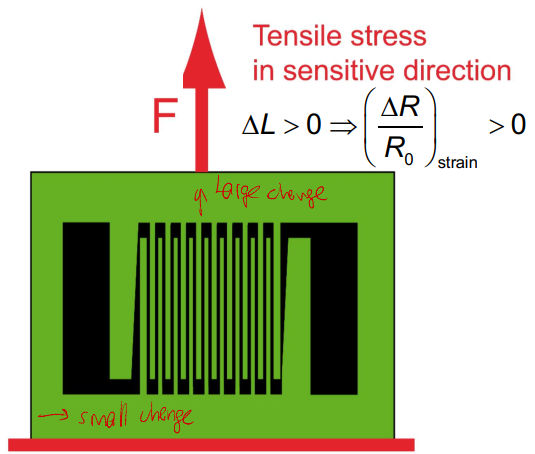
\includegraphics[width = \columnwidth]{images/strain-gauge.png}
\subsection{Readout resistive sensors}
Use a half bridge resistive divider\\
top element sensing resistor
$ \frac{v_{\text {out }}}{V_{\text {bias }}}=\frac{R}{2 R+\Delta R} \Leftrightarrow \frac{\Delta R}{R}=\frac{V_{\text {bias }}}{v_{\text {out }}}-2 $\\
Full bridge to remove offset, 2 sensing elements more sensitive,\\
remove nonlinearity by implementing differential measurements\\
Best use 4point full bridge\\
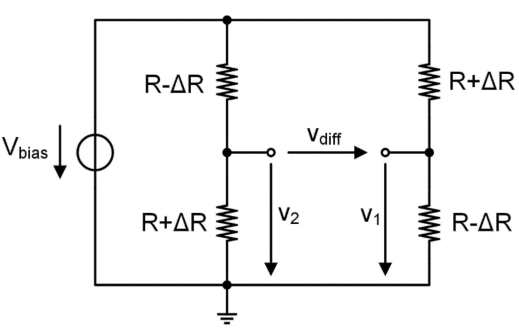
\includegraphics[width = \columnwidth]{images/4point-fullbridge.png}\\
$ V_{\mathrm{diff}}=v_{2}-v_{1}=\frac{\Delta R}{R} \cdot V_{\mathrm{bias}} $\\
Sensitivity $ S = 45mV/V$ excitation for 1V input\\
Accuracy $ A = \frac{v_{\mathrm{diff}}\left(\frac{\Delta R}{R}\right)-V_{\mathrm{diff}, \text { lin }}\left(\frac{\Delta R}{R}\right)}{V_{\mathrm{diff}}\left(\frac{\Delta R}{R}\right)} $ \\
Deviation from the ideal bridge  
\end{multicols*}
\end{document}






























